	\documentclass[11pt]{article}
	%% Packages:
\usepackage{amsmath}
\usepackage[document]{ragged2e}
\usepackage{titlesec}
\usepackage{float}
\usepackage{graphicx}
\usepackage{caption}
\usepackage{subcaption}
\usepackage[dvipsnames]{xcolor}
\usepackage[T1]{fontenc}
\usepackage{helvet}
\usepackage[hidelinks]{hyperref}
\usepackage{amssymb}
\usepackage{enumitem}
\usepackage{comment}
\usepackage{soul}
\usepackage[margin=1in]{geometry} % Set margins to 1 inch
\usepackage{setspace}
\usepackage{graphicx} % For including images
\usepackage{subcaption} % For creating subfigures
\usepackage{float} % For the [H] placement specifier
\usepackage{xcolor}
\usepackage{hyperref} % For clickable links, ToC, etc.
\usepackage{amsmath} % For math equations
\usepackage{amsfonts} % For math fonts
\usepackage{amssymb} % For math symbols
\usepackage{listings} % For code listings
\usepackage{enumitem} % For custom lists
\usepackage{booktabs} % For professional tables
\usepackage{longtable} % For tables that span multiple pages
\usepackage{array} % For more advanced table column formatting
\usepackage{fancyhdr} % For custom headers and footers
\usepackage{lastpage} % To get the total number of pages
\usepackage{csquotes} % Context sensitive quotation facilities
\usepackage{tabularx} % For tables with fixed width
\usepackage{colortbl} % For colored table cells
\usepackage{soul} % For highlighting text (use with caution)
\usepackage{tikz} % For drawing graphics directly in LaTeX
\usepackage{indentfirst}
%% Personalized adjustements: 

% Math operator:
\DeclareMathOperator{\sech}{sech}

% VUB colors: 
\definecolor{orange}{RGB}{234, 82, 0} 
\definecolor{blue}{RGB}{26, 55, 101}

% Margins:
\addtolength{\skip\footins}{0.3 cm}
\renewcommand*\footnoterule{}

% Adjustement of section, subsection & subsubsection: 

\titleformat{\section}[block]
{\normalfont\Large\bfseries \fontfamily{phv}\selectfont \color{orange}}
{\thesection}{0.5cm}{}

\titleformat{\subsection}[block]
{\normalfont\large\bfseries \fontfamily{phv}\selectfont \color{blue}}
{\thesubsection}{0.5cm}{}

\titleformat{\subsubsection}[block]
{\normalfont\small\bfseries \fontfamily{phv}\selectfont \color{blue}}
{\thesubsubsection}{0.5cm}{}
	\usepackage{setspace}
	\usepackage{graphicx}    % For including images
	\usepackage{subcaption}  % For creating subfigures
	\usepackage{float}       % For the [H] placement specifier
	\usepackage{xcolor}
	\onehalfspacing
	
	\begin{document}
		\justifying
		\begin{titlepage}
	\begin{center}
            \begin{figure}
                \centering
                
\includegraphics[scale=0.3]{Images/logo.png}
            \end{figure}
		\vspace*{\fill}
            \normalsize
            {\fontfamily{phv}\selectfont
            \textcolor{blue}{\textbf{ELEC-H404}}}\\
            \vspace{0.2cm}
		\Huge
            {\fontfamily{phv}\selectfont
            \textcolor{orange}{Advanced Security Evasion in Windows}}\\
        \end{center}
	\begin{center}	
		\vspace{0.5cm}
            \Large
            {\fontfamily{phv}\selectfont
		\textcolor{blue}{\textbf{Andranik Voskanyan\\
								Cédric Sipakam\\
								Zinar Mutlu}}}\\
	\end{center}
        \vspace*{\fill}
        \begin{FlushRight}
            {\fontfamily{phv}\selectfont
            \textcolor{orange}{Professor}}\\
            {\fontfamily{phv}\selectfont
            \textcolor{blue}{Bruno Da Silva}}\\
            \vspace{0.6cm}
%            {\fontfamily{phv}\selectfont
%            \textcolor{orange}{Teaching Assistants}}\\
%            {\fontfamily{phv}\selectfont
%            \textcolor{blue}{
%                Lucas Stefanidis\\
%                Navid Ladner 
%            }}\\
%            \vspace{0.6cm}
            {\fontfamily{phv}\selectfont
            \textcolor{orange}{Academic Year}}\\
            {\fontfamily{phv}\selectfont
            \textcolor{blue}{2024 - 2025}}\\
            \vspace{0.6cm}
            {\fontfamily{phv}\selectfont
            \textcolor{orange}{Faculty}}\\
            {\fontfamily{phv}\selectfont
            \textcolor{blue}{Electrical Engineering}}
        \end{FlushRight}



\end{titlepage}
		\tableofcontents
		\newpage
		\listoffigures
		\newpage
		
		\begin{abstract}
		This project investigates the efficacy of Windows security solutions, primarily focusing on Windows Defender, in detecting and responding to advanced stealthy attack techniques. The study evaluates a range of common attacker methodologies including the deployment of keyloggers, creation of backdoors for remote access, non-visual command execution leveraging built-in system tools, process injection for memory manipulation, and various persistence mechanisms designed to maintain unauthorized access. The evaluation involved executing these attack scenarios in a controlled environment while meticulously logging system behavior, network activity, and Windows event logs to analyze the detection capabilities and response of the security software.
		\end{abstract}
		
		\newpage
		\section{Introduction}
		\subsection{Problem Statement and Motivation}
		The Landscape of cyber threats is constantly evolving, with attackers developing increasingly sophisticated techniques to evade detection by security systems. Detecting these stealthy attacks is a significant challenge for individuals and organization alike. Understanding the methods attackers use to bypass security measures is crucial for defenders to improve their strategies, tools, and overall security posture. This project aims to shed light on these evasion techniques within the Windows operating System, a prevalent target for cyber-attacks.
		\subsection{Project Aims and Objectives}
		The Primary aims of this project are:
		\begin{itemize}
			\item To evaluate the detection capabilities of Windows Defender, [...], and [....] against a set of specific attacker techniques
			\item The attacker techniques investigated include:
				\begin{itemize}
					\item Keylogger deployment
					\item Backdoor creation and remote access
					\item Non-visual command execution and process hiding
					\item Process injection and memory manipulation
					\item Persistence techniques
				\end{itemize}
			\item To analyze system behavior, network activity, and event logs during these simulated attacks to understand how security solutions respond and what artifacts are generated
			\item To asses the effectiveness of various evasion methods employed by attackers
		\end{itemize}
		\subsection{Scope of the project}
		This project focuses on:
		\begin{itemize}
			\item \textbf{Operating System:} Windows 11 Home
			\item \textbf{Primary Security Solution:} Windows Defender, [...], [....]
			\item \textbf{Attacker Tools:} A combination of publicly available tools: Microsoft Windows Command Prompt, Netcat/Nmap, Python.
			\item \textbf{Exclusions:} This study does not cover all possible evasion techniques or every security product available on the market. The focus is on the selected methods.
		\end{itemize}
		
		
		
		
		
		\section{Background}
			\subsection{Fundamentals of Security Evasion}
			Security Evasion refers to the set of techniques and strategies employed by attacker to avoid detection by security mechanism such as antivirus software, Endpoint Detection and Response Solutions (EDR), Intrusion Detection/Prevention Systems (IDS/IPS), and firewalls. The primary goal of evasion is to allow malicious activities to proceed unnoticed, enabling attackers to achieve their objectives, which could range from data heft and espionage to system disruption or financial gain. Attacker motivations are diverse but often include maintaining stealth to ensure long-term access a.k.a persistence, escalating privileges to gain deeper system control, and exfiltrating sensitive information without triggering alarms.
			
			
			\subsection{Overview of Windows Security Architecture}
				The Windows Operating System incorporates a multi-layered security architecture designed to protect against a wide array of threats.
				\begin{itemize}
					\item \textbf{Windows Defender Antivirus:} This is the built-in anti-malware solution in Windows. Its features include:
						\begin{itemize}
							\item Real-time scanning
							\item Behavior monitoring
							\item Anti-malware Scan Interface (AMSI)
							\item Cloud-delivered protection
							\item Network Inspection System (NIS)
							\item Controlled Folder Access
						\end{itemize}
				\item \textbf{Windows Event Logging:} The OS records a wide variety of events related to system, security, application, PowerShell, and other application. Specific event IDs can indicate suspicious activities, login attempts, process creation, and security policy changes.
				\item \textbf{User Account Control (UAC):} This helps prevent unauthorized changes to the system by prompting for permission or an administrator password before performing actions that could potentially affect the computer's operation or security.
				\item \textbf{Windows Firewall:} Controls network traffic flowing in and out of the system, based on configured rules.
				\item \textbf{BitLocker Drive Encryption:} Provides full-disk encryption to protect data at rest
				\item  \textbf{AppLocker/Windows Defender Application Control (WDAC):} Allows administrators to control which applications and files users can run.
				\end{itemize}
				
				\begin{figure}[H]
					\centering
					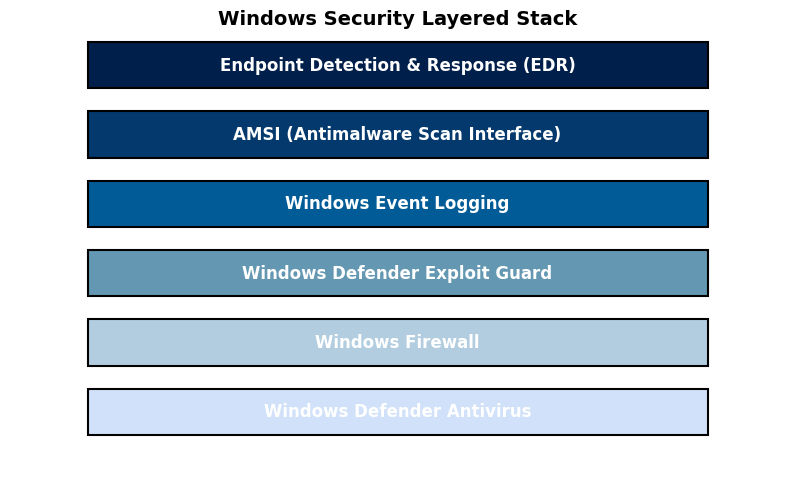
\includegraphics[width=\linewidth]{Pictures/windowssecuritylayer}
					\caption{Components of the Windows Security Architecture}
					\label{fig:windowssecuritylayer}
				\end{figure}
				
				
			\subsection{Theoretical Overview of Attacker Techniques Investigated}
				\subsubsection{Keyloggers}
				\subsubsection{Backdoors and Remote Access}
				\subsubsection{Non-Visual Command Execution and Process Hiding}
				\subsubsection{Process Injection and Memory Manipulation}
				\subsubsection{Persistence Techniques}
			\subsection{Relevant Frameworks and Tools}
			
		\section{Description}
			\subsection{Test Environment Setup}
				\subsubsection{Victim Machine}
				\subsubsection{Attacker Machine}
				\subsubsection{Network Configuration}
			\subsection{Security Solution Configuration}
				\subsubsection{Windows Defender}
			\subsection{Implementation of Attacker Techniques}
				\subsubsection{Objective of the specific test}
				\subsubsection{Tools and Scripts Used}
				\subsubsection{Step-by-step Execution Procedure}
				\subsubsection{Specific Evasion Methods Employed}
			\subsection{Monitoring and Data Collection Strategy}
				\subsubsection{Security Solution Logs}
				\subsubsection{System-Level Logs}
				\subsubsection{Network Traffic Analysis}
				\subsubsection{Performance Logging}
			\subsection{Evaluation Criteria}

		\section{Experimental Results}
			\subsection{Keylogger Deployment and Detection}
			\subsection{Backdoor Creation and Remote Access}
			\subsection{Non-Visual Command Execution and Process Hiding}
			\subsection{Process Injection and Memory Manipulation}
			\subsection{Persistence Techniques}
			\subsection{Security Solution Performance Analysis}
			\subsection{Comparative Analysis}
			
		\section{Discussion and Conclusion}
			\subsection{Interpreation of Results}
			\subsection{Comparison with Expected Outcomes/Litterature}
			\subsection{Challenges Encountered and Limitations of the Study}
			\subsection{Conclusion}
			\subsection{Future Perspectives}
			
		\section{References}
		
	\end{document}